\documentclass[12pt,a4paper]{report}

\usepackage[a4paper,margin=1in]{geometry}
\usepackage[T1]{fontenc}
\usepackage[utf8]{inputenc}
\usepackage{newtxtext,newtxmath}
\usepackage{setspace}
\usepackage{graphicx}
\graphicspath{{figures/}}
\usepackage{booktabs}
\usepackage{array}
\usepackage{longtable}
\usepackage{tabularx}
\usepackage{float}
\usepackage{caption}
\usepackage{subcaption}
\usepackage{amsmath}
\usepackage{enumitem}
\usepackage{titlesec}
\usepackage{fancyhdr}
\usepackage{hyperref}
\usepackage{url}
\usepackage{cite}
\usepackage{xcolor}
\usepackage{listings}

\hypersetup{
    colorlinks=true,
    linkcolor=black,
    citecolor=black,
    urlcolor=blue
}

\setlength{\parindent}{0pt}
\setlength{\parskip}{0.4em}
\setlist{topsep=0.35em,itemsep=0.2em,parsep=0pt,partopsep=0pt}
\onehalfspacing

\titleformat{\chapter}[display]
{\bfseries\centering\Large}
{Chapter \thechapter}
{0.5em}
{\Large}

\titleformat{\section}
{\bfseries\normalsize}
{\thesection}
{0.75em}
{}

\titleformat{\subsection}
{\bfseries\normalsize}
{\thesubsection}
{0.75em}
{}

\pagestyle{fancy}
\fancyhf{}
\fancyhead[R]{\thepage}
\renewcommand{\headrulewidth}{0pt}

\lstset{
    language=Python,
    basicstyle=\ttfamily\small,
    breaklines=true,
    frame=single,
    columns=fullflexible,
    keepspaces=true,
    showstringspaces=false
}

\DeclareRobustCommand{\codefile}[1]{\texttt{\detokenize{#1}}}
\newcommand{\pathcell}[2]{\shortstack[l]{\codefile{#1}\\\codefile{#2}}}

\begin{document}

\begin{titlepage}
    \thispagestyle{empty}
    \begin{center}
        \vspace*{0.8cm}
        
\includegraphics[width=0.5\linewidth]{ntu_logo.png}\\[3.2cm]
        {\large PCCDS24-0086\par}
        \vspace{0.35cm}
        {\bfseries
        \large Scenario Generation Methods for Functional Safety Testing of Automated Driving Systems\par}
        \vspace{1.4cm}
        {\large Submitted by: Chaw Kay Khine\par}
        \vspace{2.3cm}
        {\normalsize Supervisor: Prof Liu Yang\par}
        \vspace{0.25cm}
        {\normalsize Co-supervisor: Wen Bing\par}
        \vspace{1.8cm}
        {\normalsize School of Computer Science and Engineering\par}
        \vspace{1.6cm}
        {\normalsize A final year project report presented to Nanyang Technological University\par}
        \vspace{0.2cm}
        {\normalsize in partial fulfilment of the requirements for the\par}
        \vspace{0.2cm}
        {\normalsize Degree of Bachelor of Engineering\par}
        \vfill
        {\normalsize 2024/2026\par}
    \end{center}
\end{titlepage}

\pagenumbering{roman}

\chapter*{Abstract}
\addcontentsline{toc}{chapter}{Abstract}
Automated driving systems must be evaluated under a large number of traffic situations before any safety claim can be taken seriously. Real-world testing alone is too slow, too costly, and too risky for this purpose. Scenario-based simulation is therefore an important engineering tool because it allows the same driving task to be repeated under controlled conditions while traffic, road layout, and dynamic events are changed in a measurable way.

This project develops a simulation-based evaluation framework in MetaDrive for three different scenario classes: highway, intersection-roundabout, and street driving with pedestrians. The work started from a practical question rather than a purely theoretical one: if several built-in and modified driving policies are tested under the same repeatable conditions, which policy is most suitable for each scenario, and what kind of failure does each policy show? To answer that question, the project implements custom scenario logic, policy assignment, episode logging, workbook export, and notebook-based analysis.

The most important part of the work lies in Chapters 4, 5, and 6, where the system design, implementation logic, and experimental findings are explained in detail. The report shows how the ideas developed through the project process. On the highway, poor Expert-policy progress motivated a hybrid recovery design using IDM fallback. In the intersection-roundabout case, lack of route control motivated a custom fixed-route map and target-only trajectory assignment. In the street case, the need to evaluate vulnerable road users motivated a multi-crosswalk event pipeline and a pedestrian-aware extension of IDM.

The final results show that policy performance is strongly scenario-dependent. Plain IDM is the strongest overall baseline in the highway and intersection datasets because it gives the best balance of completion and control stability. In the street scenario, the project-authored Hybrid IDM policy gives the best balance between route completion and pedestrian safety, although it still needs improvement in vehicle-to-vehicle interaction. The report therefore concludes that scenario-specific engineering is necessary, and that pass rate alone is not enough for safety-oriented evaluation. Timeout behaviour, crash type, speed, and time-to-goal must all be considered together.

\chapter*{Acknowledgment}
\addcontentsline{toc}{chapter}{Acknowledgment}
I would like to express my sincere gratitude to my supervisor, Prof Liu Yang, for giving me the opportunity to carry out this project and for his support throughout the research process.

I am deeply thankful to my co-supervisor, Wen Bing, for his technical guidance, practical advice, and support during the implementation of the MetaDrive simulator framework. His assistance in system design, debugging, and experiment setup was important to the completion of this work.

I would also like to acknowledge the MetaDrive development team and the wider open-source community for providing a useful platform for autonomous driving research. Their documentation and shared resources made this project possible.

Finally, I would like to thank the School of Computer Science and Engineering at Nanyang Technological University for providing the academic environment and resources required for this final year project.

\bigskip
\begin{flushright}
Chaw Kay Khine \quad March 2026
\end{flushright}

\tableofcontents
\listoffigures
\listoftables

\clearpage
\pagenumbering{arabic}

\chapter{Introduction}

\section{Background and Motivation}
Automated driving systems are expected to operate with an acceptable level of safety in complex and changing traffic environments. In engineering practice, this expectation is discussed in relation to functional safety, safety of the intended functionality, and structured validation processes \cite{iso26262,iso21448,sae3016,unece_natm}. A successful demonstration is not enough. The system must be examined across many traffic situations, especially those that are difficult, uncommon, or safety-critical.

For this reason, simulation has become an important part of automated driving research and development. Simulation allows the same driving task to be repeated while road layout, traffic interaction, and event timing are varied in a controlled way \cite{wang2024scenario,zhang2024virtual,skoglund2025safety}. This improves repeatability, reduces cost, and makes it possible to investigate situations that would be difficult or unsafe to reproduce directly on public roads.

The motivation of this project comes from general technical curiosity about how different driving algorithms behave under different scenario types. A method that appears effective in one environment may not behave equally well in another. This raises a broader research interest: how should scenario-based experiments be designed so that behaviour can be observed fairly, failure modes can be explained clearly, and conclusions can be supported with traceable evidence \cite{wang2024scenario,song2023critical}?

\section{Problem Statement}
Scenario-based testing is a standard way to study autonomous driving behaviour, but the scenario space is very large. Even when only one simulator is used, the combination of road structure, spawn location, surrounding traffic, obstacles, and event timing grows quickly. If the experiment design is weak, several problems appear:

\begin{enumerate}[label=\arabic*.]
    \item different algorithmic approaches may not face exactly the same task,
    \item the recorded output may hide the actual failure mode,
    \item a high pass rate may give a misleading impression if timeout and crash information are ignored, and
    \item the conclusions may not generalize even across different kinds of simulated road context.
\end{enumerate}

The project therefore addresses the following practical problem: how can a repeatable simulation-based framework be designed so that multiple algorithmic approaches can be compared fairly across different classes of driving scenario, while still producing evidence detailed enough for a functional-safety-oriented engineering report \cite{wang2024scenario,song2023critical,skoglund2025safety}?

\section{Aim and Objectives}
\subsection*{Aim}
The aim of this project is to support functional-safety-oriented discussion for automated driving by building a repeatable simulation-based evaluation framework and using it to compare controller behaviour across multiple scenario types.

\subsection*{Objectives}
The main objective is to develop, implement, and assess an autonomous driving simulation framework for comparative evaluation of different driving algorithms under highway, intersection, and street scenarios.

\vspace{0.5em}
The specific objectives are:
\begin{enumerate}[label=\arabic*.]
    \item To create and configure three representative simulation scenarios covering different categories of road interaction.
    \item To implement and test several algorithmic approaches for autonomous driving.
    \item To introduce scenario-specific mechanisms where necessary, such as fixed-route multi-agent behaviour and pedestrian-crossing events.
    \item To collect, export, and organise repeated episode data for later analysis.
    \item To evaluate comparative performance using completion rate, timeout rate, crash indicators, speed, and travel time.
    \item To identify the most suitable algorithmic approach for each scenario and explain the reason using the recorded evidence.
\end{enumerate}

\section{Research Questions}
The report is guided by four research questions.

\begin{enumerate}[label=\textbf{RQ\arabic*.}]
    \item How does the ranking of algorithmic approaches change when the scenario changes from highway driving to structured conflict points and then to pedestrian interaction?
    \item Can relatively simple reactive algorithms outperform more complex algorithmic approaches in some scenarios?
    \item Can scenario-specific engineering changes solve a clear failure mode observed during development?
    \item Which combination of metrics gives the most honest interpretation of comparative algorithmic performance in this project?
\end{enumerate}

\section{Research Evolution}
The project did not begin with a fixed platform choice. The initial implementation work was carried out in SUMO for mixed-traffic analysis \cite{sumo,sumo_docs}. That stage was useful for understanding traffic interaction, but several limitations became clear when the work shifted toward richer scenario representation and a stronger functional-safety framing:

\begin{itemize}
    \item the two-dimensional presentation was less suitable for final report documentation,
    \item scenario construction was less convenient for the type of custom safety-oriented tasks needed here,
    \item direct support for integrated episode-level safety monitoring required more additional development, and
    \item the overall workflow was not as well matched to the type of controller comparison this project needed.
\end{itemize}

\begin{figure}[H]
    \centering
    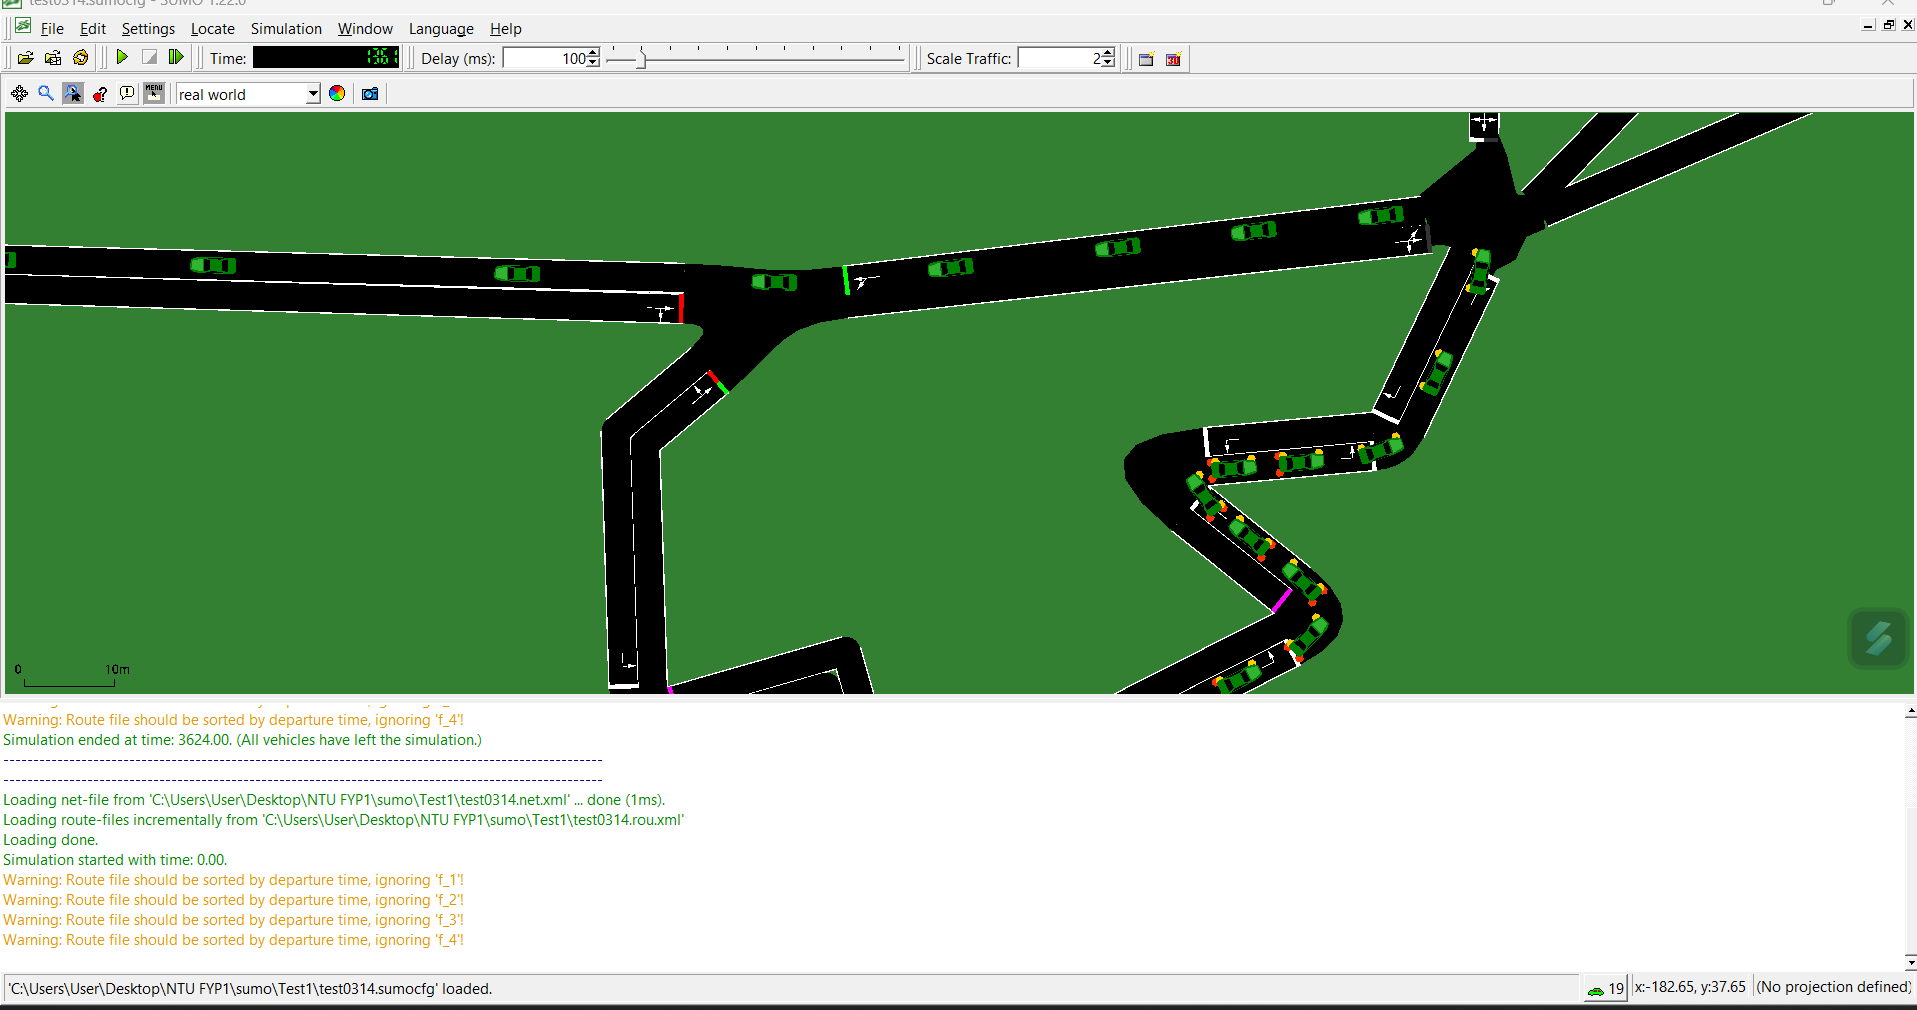
\includegraphics[width=0.82\textwidth]{sumo_2d_visualization.png}
    \caption{Initial work in SUMO. The platform was useful for traffic analysis, but not the best final choice for the kind of project-specific three-dimensional scenario evaluation required in this report.}
    \label{fig:sumo_2d}
\end{figure}

As the project developed, higher-fidelity three-dimensional simulation platforms were explored as part of the selection process \cite{zhang2024virtual,carla,carla_official}. The final platform decision was made only after the project requirements had become clearer, especially with respect to scenario flexibility, iteration speed, and the need for a controlled evaluation workflow.

\section{Main Contributions of the Project}
The final contribution is not only a set of simulation videos. The project delivers an end-to-end evaluation framework with the following main contributions:

\begin{enumerate}[label=\arabic*.]
    \item A repeatable highway evaluation setup with fixed road structure.
    \item A custom intersection-roundabout map and route-management pipeline for fair multi-agent comparison.
    \item A street scenario with repeated pedestrian-crossing events injected along the ego route.
    \item Project-authored control refinements targeting identified failure modes.
    \item Workbook-based experiment logging and notebook-based comparative analysis.
    \item Scenario-specific findings that show why a single controller family does not dominate every road context.
\end{enumerate}

\section{Report Structure}
\begin{itemize}
    \item Chapter 2 reviews the background literature and technical concepts relevant to the project.
    \item Chapter 3 presents the research methodology, platform selection process, and evaluation metrics.
    \item Chapter 4 explains the system design and the rationale behind the scenario architecture.
    \item Chapter 5 describes the implementation in detail, including representative code logic and experiment execution.
    \item Chapter 6 presents the final results and discusses the findings on a scenario-by-scenario basis.
    \item Chapter 7 concludes the report and summarises the main lessons, limitations, and future work.
\end{itemize}

\chapter{Literature Review}

\section{Simulation-Based Testing for Automated Driving}
Road testing gives realism, but it scales poorly for rare or hazardous situations. Simulation is therefore used to extend coverage, increase repeatability, and make controlled comparison possible. In scenario-based testing, the system is not evaluated through one undifferentiated long drive. Instead, it is evaluated through a set of designed situations that represent important forms of interaction such as lane following, junction crossing, yielding, and hazard response \cite{unece_natm,wang2024scenario,skoglund2025safety}.

For this project, scenario-based testing is important for two reasons. First, it allows the same controller to be evaluated under different road structures. Second, it allows the report to study failure behaviour directly. If a controller stops, times out, or accumulates crashes, the cause can be linked to a specific kind of scenario rather than hidden inside one large generic test.

\section{Functional Safety and Safety of the Intended Functionality}
ISO 26262 is widely used when discussing structured functional safety processes for road vehicles \cite{iso26262}. ISO 21448 addresses risk that arises when the system behaves as designed but still does not handle the environment safely enough \cite{iso21448}. SAE J3016 provides shared terminology for levels of driving automation and related concepts \cite{sae3016}.

This project does not attempt to perform full industrial certification. However, the motivation of the work is aligned with safety-oriented engineering practice: the controller should not only complete the route, but should do so with behaviour that is measurable, explainable, and comparable across conditions.

\section{Scenario Generation Methods}
Scenario generation methods can be grouped broadly into rule-based, data-driven, search-based, and compositional approaches \cite{wang2024scenario,song2023critical,openscenario_standard}. Rule-based methods rely on engineering constraints and known traffic logic. Data-driven methods build scenarios from recorded driving data. Search-based methods try to find parameter combinations that stress the controller. Compositional methods build larger scenarios by combining smaller map blocks or event elements.

The present project is closest to a compositional and rule-guided approach. The road structure is built procedurally, but the main scenarios are not random in a fully open-ended sense. They are deliberately constrained so that algorithmic approaches can be compared on a fixed task. This design choice is appropriate for a final year engineering report because it reduces uncontrolled variation and makes the conclusions easier to defend.

\section{Representative Control Approaches in Automated Driving Research}
Several control approaches are commonly explored in automated driving research and simulation:

\begin{itemize}
    \item \textbf{Reactive car-following control.} These methods respond directly to nearby traffic states and are often valued for simplicity and interpretability.
    \item \textbf{Rule-based or expert-inspired control.} These methods use predefined logic, route information, and behavioural rules to guide the vehicle.
    \item \textbf{Trajectory-guided control.} These methods follow an explicit reference path and are useful when route structure is known in advance.
    \item \textbf{Learning-based control.} These methods optimise behaviour from reward or data, and are often explored when hand-designed rules become too limited.
\end{itemize}

In practice, these categories are not mutually exclusive. Hybrid solutions are often used, especially when a baseline method performs well in general but requires additional logic to handle a specific safety-related weakness.

\section{Simulation Platforms for Scenario-Based Evaluation}
The simulator had to satisfy several requirements: support for three-dimensional rendering, custom scenario creation, policy-level control, manageable compute cost, and convenient repeated evaluation. Table~\ref{tab:platform_compare} summarises the practical comparison that guided the platform decision.

\begin{table}[H]
    \centering
    \small
    \caption{Practical platform comparison for this project}
    \label{tab:platform_compare}
    \begin{tabularx}{\textwidth}{>{\raggedright\arraybackslash}p{2.7cm} X X X}
        \toprule
        Criterion & SUMO & CARLA & MetaDrive \\
        \midrule
        Visual presentation & Mainly two-dimensional & High-fidelity three-dimensional scenes & Lightweight three-dimensional simulation \\
        Route-level customisation & Good for traffic studies & Strong, but heavier to set up and run & Strong and easy to extend inside Python \\
        Built-in policy experimentation & Limited for this project focus & Possible, but more expensive to iterate & Well matched to controller comparison \\
        Procedural scenario generation & Limited for this project goal & Good, but heavier infrastructure & Strong compositional map generation \\
        Iteration speed under project constraints & Strong & Weaker under limited resources & Strong \\
        Suitability for final report evidence & Moderate & Strong & Strong \\
        \bottomrule
    \end{tabularx}
\end{table}

\section{Selection of the Final Simulation Platform}
MetaDrive was selected because it gave the best balance between scenario control and development speed \cite{metadrive,metadrive_docs,metadrive_github}. The project needed to do more than run a standard demo. It needed to:

\begin{enumerate}[label=\arabic*.]
    \item build custom map structures,
    \item assign different policies to ego and traffic vehicles,
    \item extend policy logic directly in Python,
    \item inject dynamic events such as pedestrian crossing, and
    \item export repeated results for analysis.
\end{enumerate}

MetaDrive supports all of these requirements within one codebase. This made it suitable not only for experimentation, but also for a report that had to explain the full engineering process from idea formation to final findings.

\chapter{Research Methodology and Platform Selection}

\section{Research Methodology Overview}
The methodology of the project follows a clear sequence:

\begin{enumerate}[label=\arabic*.]
    \item identify the evaluation question,
    \item design a scenario that isolates that question,
    \item connect one algorithmic approach at a time to the ego vehicle,
    \item run repeated episodes under fixed settings,
    \item log the outputs to spreadsheets, and
    \item analyse the compiled results with notebook-based plots and summary statistics.
\end{enumerate}

This sequence is important because it turns a simulator repository into a real engineering workflow. The final report is based on that workflow, not only on informal visual inspection.

\section{Selection of Scenario Classes}
The three scenarios were selected because they stress different parts of driving behaviour.

\begin{table}[H]
    \centering
    \small
    \caption{Purpose of the three scenario classes}
    \label{tab:scenario_purpose}
    \begin{tabularx}{\textwidth}{>{\raggedright\arraybackslash}p{2.8cm} X X}
        \toprule
        Scenario & Main behaviour under test & Main failure that the scenario can reveal \\
        \midrule
        Highway & Longitudinal progress, obstacle response, lane-level interaction & Stagnation behind traffic, inability to recover, collision accumulation during overtaking or blockage \\
        Intersection-roundabout & Conflict-point negotiation, route control, multi-agent interaction & Over-cautious behaviour, route-tracking weakness, unsafe crossing at structured conflicts \\
        Street with pedestrians & Yielding to vulnerable road users while still making progress & Pedestrian contact, excessive freezing, poor balance between safety and mobility \\
        \bottomrule
    \end{tabularx}
\end{table}

Using only one scenario would have hidden the central finding of the project, which is that the ranking of algorithmic approaches changes significantly with context.

\section{Experimental Control and Comparison Fairness}
The project uses fixed route definitions wherever possible. This is a key methodological choice. If the route changes from run to run, it becomes difficult to tell whether the result difference comes from the algorithm or from the task itself. For this reason:

\begin{itemize}
    \item the highway scenario uses a fixed map string and fixed ego spawn lane,
    \item the intersection-roundabout scenario fixes the target route through a custom map and spawn manager, and
    \item the street scenario fixes the map and spawn lane, then inserts pedestrian events at known route fractions.
\end{itemize}

These controls make the comparative evaluation more defensible.

\section{Performance Metrics}
The project does not rely on one final score. Several metrics are logged because each metric answers a different question.

\begin{align}
\text{Pass rate} &= \frac{N_{\text{pass}}}{N_{\text{episodes}}}\times 100\% \\
\text{Timeout rate} &= \frac{N_{\text{timeout}}}{N_{\text{episodes}}}\times 100\% \\
\text{Mean crash count} &= \frac{\sum_{i=1}^{N} c_i}{N}
\end{align}

Average speed and time-to-goal are then used to judge whether an algorithmic approach succeeded efficiently or only by moving too slowly.

\subsection*{Meaning of each metric}
\begin{itemize}
    \item \textbf{Pass} indicates that the policy completed the scenario under the logging rule used by that script.
    \item \textbf{Timeout} indicates that the vehicle stopped making enough progress.
    \item \textbf{Crash count} captures unsafe interaction, but the type of crash also matters.
    \item \textbf{Average speed} captures movement quality over the episode.
    \item \textbf{Time to goal} measures route efficiency for successful episodes.
\end{itemize}

\section{Data Processing and Analysis Pipeline}
The raw result files produced by the batch scripts are stored in scenario-specific folders. Those files are then consolidated into three main workbooks:

\begin{itemize}
    \item \codefile{highway_analysis_compilation.xlsx},
    \item \codefile{Intersection_analysis_compilation.xlsx}, and
    \item \codefile{street_analysis_compilation.xlsx}.
\end{itemize}

Jupyter notebooks then load the compiled sheets and produce the final summary figures used in the report. One useful detail is that the highway workbook stores time-to-goal values as \texttt{mm:ss} text, while the notebook converts them to seconds for analysis. This kind of data-handling step is small, but it matters if the report is to match the saved workbook correctly.

\section{Methodological Constraints}
Even before the final results are discussed, several limitations are already visible at the methodology stage:

\begin{enumerate}[label=\arabic*.]
    \item sample sizes are not fully equal across every policy,
    \item some policy variants were implemented but not included in the final consolidated benchmark,
    \item the street scripts do not all use exactly the same timeout rule, and
    \item the project remains fully simulation-based.
\end{enumerate}

These limitations do not remove the value of the work, but they must be stated openly so that the conclusions are read correctly.

\chapter{System Design}

This chapter explains how the evaluation framework was designed before the code-level implementation is discussed. The design is important because the project was not built as a collection of unrelated scripts. It was built to answer specific questions in a repeatable way.

\section{Design Objectives}
The design of the framework was driven by four practical questions.

\begin{enumerate}[label=\arabic*.]
    \item If the same controller family is moved across very different road contexts, does its ranking remain stable?
    \item When a baseline policy shows an obvious weakness, can a simple engineering modification improve it?
    \item Which part of the system should be changed when performance is poor: the route design, the event logic, or the controller itself?
    \item What does each metric reveal that a simple pass or fail label would miss?
\end{enumerate}

These questions directly shaped the architecture and the final scenario selection.

\section{Design Principles}
Four design principles were used throughout the project.

\subsection*{Repeatability}
Every policy should face the same scenario definition. This is why fixed route logic and fixed spawn rules were used wherever possible.

\subsection*{Progressive difficulty}
The scenarios were arranged so that the interaction difficulty increases from highway flow, to structured conflict points, to repeated pedestrian events.

\subsection*{Traceability}
Every episode should produce a row that can be traced back to a scenario, a policy, and a batch script.

\subsection*{Targeted modification}
When a baseline failed, the response should solve the observed failure rather than replace everything without explanation.

\section{Overall Architecture}
The full system can be understood as four connected layers.

\begin{enumerate}[label=\textbf{L\arabic*:}, leftmargin=2.2cm]
    \item \textbf{Scenario layer.} Defines map structure, traffic, obstacles, dynamic events, and end conditions.
    \item \textbf{Policy layer.} Assigns the control logic used by the ego vehicle and, where needed, traffic vehicles.
    \item \textbf{Execution layer.} Steps the environment, monitors status, handles timeout logic, and collects runtime information.
    \item \textbf{Data layer.} Writes episode summaries, consolidates them into workbooks, and feeds the notebook analysis stage.
\end{enumerate}

\begin{figure}[H]
    \centering
    \fbox{\parbox{0.9\textwidth}{\centering\vspace{0.6em}
    \textbf{Scenario design} $\rightarrow$ \textbf{Policy execution} $\rightarrow$ \textbf{Step monitoring} $\rightarrow$ \textbf{Episode logging} $\rightarrow$ \textbf{Workbook compilation} $\rightarrow$ \textbf{Notebook analysis}\vspace{0.6em}}}
    \caption{Logical workflow shared by all experiments in the project}
    \label{fig:workflow}
\end{figure}

\section{Scenario-Specific Design Rationale}
Although all three scenarios live inside the same simulator ecosystem, they were not designed in the same way. The reason is that each scenario is intended to expose a different class of failure.

\begin{table}[H]
    \centering
    \small
    \caption{Design intention of each scenario}
    \label{tab:design_intention}
    \begin{tabularx}{\textwidth}{>{\raggedright\arraybackslash}p{2.6cm} X X X}
        \toprule
        Scenario & Main design choice & Why that choice was needed & Main evidence expected \\
        \midrule
        Highway & Fixed map string with traffic and accidents & To test continuous progress under blockage and mixed traffic & Completion, timeout, and collision burden \\
        Intersection-roundabout & Custom block chain and fixed target route & To prevent route randomness from hiding policy differences & Junction completion, conflict handling, route efficiency \\
        Street & Crosswalk injection and staged pedestrian events & To test repeated vulnerable-road-user interaction along one route & Pedestrian safety, progress, and vehicle interaction trade-off \\
        \bottomrule
    \end{tabularx}
\end{table}

\section{Highway Scenario Design}
The highway scenario was designed around a clear engineering question: if the ego vehicle is placed on a fixed highway route with mixed traffic and accident-related obstacles, which controller can continue making progress without becoming trapped or colliding excessively?

\subsection{Fixed Route Representation}
The map string \texttt{CSrRSY\$yRSCR} was used because it gave a stable route with meaningful highway behaviour, including ramps and split or merge structure. Using a fixed map string keeps the road structure constant, so the analysis focuses on controller behaviour rather than map randomness.

\subsection{Traffic and Obstacle Configuration}
If the highway were empty, the test would mainly measure route following. That was not enough. Traffic density, inverse traffic, random traffic, accident probability, and static traffic objects were enabled so that the controller had to deal with congestion, blocked progress, and collision risk. This makes the scenario more suitable for a safety-oriented discussion.

\subsection{Safety-Oriented Environment Selection}
\texttt{SafeMetaDriveEnv} provides a suitable loop for monitoring road safety conditions. It gives convenient access to crash and episode information, which simplifies evaluation and logging.

\section{Intersection-Roundabout Scenario Design}
The intersection-roundabout scenario was designed to answer a different question: if the route is short but contains several conflict points, does explicit route structure help, and how do policies trade speed against crash behaviour?

\subsection{Necessity of Explicit Map Construction}
The project needed \texttt{agent0} to start from the same road and finish at the same roundabout exit every time. A one-line procedural map string did not give enough direct control for that goal. A custom map was therefore built from four explicit blocks:

\begin{enumerate}[label=\arabic*.]
    \item \texttt{FirstPGBlock},
    \item \texttt{InterSection},
    \item \texttt{Straight},
    \item \texttt{Roundabout}.
\end{enumerate}

This design makes the ego route transparent and reproducible.

\subsection{Multi-Agent Interaction Design}
The scenario is not meant to test route following in an empty road. Interruption vehicles are spawned on other roads so that the ego vehicle must deal with crossing and merging traffic. This allows the experiment to study both completion and conflict behaviour.

\section{Street Scenario Design}
The street scenario was designed around the most safety-critical interaction in the project: vehicle behaviour around pedestrians.

\subsection{Repeated Crosswalk Event Design}
One pedestrian event near the start of the route would not be enough to show whether the controller can recover and continue safely. The street map therefore injects crosswalks at route fractions \texttt{0.34}, \texttt{0.56}, and \texttt{0.78}. This means the ego vehicle meets pedestrians repeatedly during the same episode.

\subsection{Event Sequencing Strategy}
The goal was not to create uncontrolled chaos. Each crosswalk event is allowed to finish before the next one begins. This design improves interpretability. If the controller fails, the failure can be related more clearly to a specific interaction stage.

\subsection{Traffic Density Selection}
The traffic density was kept around six to seven traffic vehicles so that the street task still remained readable. If dense traffic and repeated pedestrians were both maximised at the same time, it would be harder to explain which factor caused the policy to fail.

\section{Policy Ownership and Comparison Strategy}
The report distinguishes clearly between baseline policies and project-authored additions.

\begin{table}[H]
    \centering
    \small
    \caption{Policy ownership in the project}
    \label{tab:policy_ownership}
    \begin{tabularx}{\textwidth}{>{\raggedright\arraybackslash}p{3.4cm} X X}
        \toprule
        Policy or component & Ownership status & Role in the project \\
        \midrule
        \texttt{IDMPolicy} & MetaDrive baseline & Reactive baseline for comparison \\
        \texttt{ExpertPolicy} & MetaDrive baseline & Expert-style baseline for comparison \\
        \texttt{TrajectoryIDMPolicy} & MetaDrive baseline & Route-following baseline for comparison \\
        \texttt{StuckAwareExpertPolicy} & Project-authored wrapper & Highway recovery policy for Expert stagnation \\
        \texttt{ObstacleAwareTrajectoryIDMPolicy} & Project-authored wrapper & Highway trajectory policy with reactive avoidance mode \\
        Intersection custom map and managers & Project-authored implementation & Fixed-route multi-agent evaluation environment \\
        Street crosswalk and pedestrian event pipeline & Project-authored implementation & Repeated pedestrian interaction testbed \\
        \texttt{PedestrianAwareIDMPolicy} & Project-authored policy extension & Street controller with pedestrian-aware braking and steering logic \\
        PPO training script & Project-authored training workflow & Exploration of learned optimisation on the custom intersection route \\
        \bottomrule
    \end{tabularx}
\end{table}

\section{Design Evolution and Engineering Rationale}
An important part of the final report is not only what was built, but why each idea appeared. Table~\ref{tab:idea_evolution} summarises that development process.

\begin{table}[H]
    \centering
    \small
    \caption{How observations during development led to design ideas}
    \label{tab:idea_evolution}
    \begin{tabularx}{\textwidth}{>{\raggedright\arraybackslash}p{3.1cm} X X}
        \toprule
        Observation during development & Design idea introduced & Reasoning \\
        \midrule
        Expert policy stalled badly on the highway & Add IDM fallback after clear non-progress signals & A recovery rule is simpler and more explainable than replacing the controller completely \\
        The highway route is known but local interaction still matters & Add trajectory following with reactive fallback mode & Planned motion may help route stability, but interaction still needs a reactive escape mechanism \\
        Intersection comparison was unfair if the route could change & Build a fixed-route custom map and spawn manager & Route randomness would hide policy differences \\
        Street testing needed repeated pedestrian interaction, not just one event & Inject three crosswalk sites along the route & The controller should show safe behaviour repeatedly over one trip \\
        Street IDM was safe but too hesitant, while Expert was efficient but pedestrian-unsafe & Extend IDM with pedestrian conflict logic & The goal was to improve safety and still keep the route moving \\
        \bottomrule
    \end{tabularx}
\end{table}

\section{Data Flow and Traceability}
The design deliberately produces one row per episode. This is a strong choice for traceability. It means the report can move from raw simulation behaviour to summary plots without re-running the simulator. It also means that every conclusion in Chapter 6 can be connected back to a saved workbook, a sheet, and a policy.

\chapter{Detailed Implementation and Experimental Procedure}

This chapter explains how the design from Chapter 4 was translated into code. The emphasis is on important implementation logic, why that logic matters, and how it connects to the experiment outputs used later in the report.

\section{Implementation Structure}
The main implementation work is grouped by scenario under the \codefile{test/Final analysis/} directory.

\begin{table}[H]
    \centering
    \small
    \caption{Main implementation groups used in the project}
    \label{tab:repo_groups}
    \begin{tabularx}{\textwidth}{>{\raggedright\arraybackslash}p{4.0cm} X}
        \toprule
        Folder or script group & Main role in the project \\
        \midrule
        \pathcell{Final analysis/Highway analysis/}{highway\_IDM.py, highway\_Expert+IDM.py, highway\_Trajectory.py} & Highway environment setup, policy logic, and repeated testing \\
        \pathcell{Final analysis/Intersection analysis/}{intersection\_IDM.py, intersection\_EXPERT.py, intersection\_TrajectoryIDM.py} & Custom route environment, target-agent control, and intersection evaluation \\
        \pathcell{Final analysis/Street analysis/}{street\_expert.py, street\_IDM.py, street\_HybridIDM.py} & Street scenario generation, crosswalk logic, and street policy comparison \\
        \pathcell{backup files/}{train\_optimized\_policy.py} & PPO training workflow for the custom intersection route \\
        \bottomrule
    \end{tabularx}
\end{table}

\section{Common Experimental Workflow}
Although the scenarios are different, the high-level experiment pattern is the same in all of them:

\begin{enumerate}[label=\arabic*.]
    \item build the environment with fixed settings,
    \item attach the chosen policy to the ego vehicle,
    \item reset and run one episode,
    \item monitor the episode step by step,
    \item save one summary row for that run,
    \item repeat for multiple episodes, and
    \item export the results to Excel for later analysis.
\end{enumerate}

This consistency is valuable because it means the comparison changes the policy or the scenario, not the overall experiment logic.

\section{Highway Implementation}

\subsection{Highway Environment Configuration}
The highway scripts are built on \texttt{SafeMetaDriveEnv}. The core settings are intentionally fixed: the ego vehicle always spawns on the same lane, the map string stays constant, and the traffic conditions stay within one chosen range.

\begin{lstlisting}[caption={Representative highway configuration logic.},label={lst:highway_config},float=H]
env = SafeMetaDriveEnv(
    dict(
        agent_policy=IDMPolicy,
        map="CSrRSY$yRSCR",
        traffic_density=0.05,
        need_inverse_traffic=True,
        random_traffic=True,
        accident_prob=0.25,
        static_traffic_object=True,
        horizon=5000,
        random_spawn_lane_index=False,
        vehicle_config={
            "spawn_lane_index": (FirstPGBlock.NODE_2, FirstPGBlock.NODE_3, 0)
        },
    )
)
\end{lstlisting}

Conceptually, this configuration is important because it creates a controlled but non-trivial highway task. The ego vehicle is not driving on an empty road. It must continue moving through traffic and accident-related blockage.

\subsection{Baseline Highway Controllers}
Three baseline controller families appear in the highway work:

\begin{itemize}
    \item \texttt{IDMPolicy},
    \item \texttt{ExpertPolicy}, and
    \item \texttt{TrajectoryIDMPolicy}.
\end{itemize}

The baseline tests answer the first question: how far can the built-in policies go without project-specific modification?

\subsection{Rationale for the Highway Recovery Controller}
During development, one of the clearest observations was that the Expert policy could remain almost stationary for long periods on the tested highway. That observation directly motivated a recovery design. The idea was not to remove Expert completely, but to let Expert operate until strong evidence of non-progress appeared.

\begin{lstlisting}[caption={Core recovery logic of the highway Expert+IDM policy.},label={lst:expert_idm_logic},float=H]
class StuckAwareExpertPolicy(ExpertPolicy):
    SLOW_SPEED_KMH = 8.0
    SLOW_CONSECUTIVE_STEPS = 10
    STUCK_DIST_M = 3.0
    STUCK_WINDOW_STEPS = 30

    def act(self, agent_id=None):
        if self._use_fallback:
            return self._get_fallback_policy().act(agent_id)

        if speed_kmh < self.SLOW_SPEED_KMH:
            self._slow_count += 1
        else:
            self._slow_count = 0

        if self._slow_count >= self.SLOW_CONSECUTIVE_STEPS:
            return self._trigger_idm("speed-based stuck detection")

        if moved_distance_in_window < self.STUCK_DIST_M:
            return self._trigger_idm("position-based stuck detection")

        return super().act(agent_id)
\end{lstlisting}

This logic can be explained theoretically as a supervisory hybrid controller. Expert remains the primary policy, but a higher-level supervisor monitors progress. If the progress state becomes unacceptable, control is transferred to IDM. Two detection modes are used because speed alone may miss slight movement, and displacement alone may react too late.

\subsection{Rationale for the Highway Trajectory-Based Controller}
The trajectory variant explores a different idea. Instead of driving only through local reaction, the ego vehicle is given a reference path created from the road network. However, a pure route-following policy can still become blocked. The project therefore adds a mode switch between path-following and reactive avoidance.

\begin{lstlisting}[caption={Simplified logic of the highway trajectory variant.},label={lst:traj_logic},float=H]
def _build_trajectory_point_lane(road_network, spawn_lane_index, dest_node):
    path = road_network.shortest_path(spawn_lane_index, dest_node)
    path_points = concatenate_lane_polylines(path)
    return PointLane(path_points, lane_width=2.0)

class ObstacleAwareTrajectoryIDMPolicy(TrajectoryIDMPolicy):
    STUCK_SPEED_KMH = 2.0
    STUCK_STEPS = 30
    RESUME_SPEED_KMH = 8.0
    RESUME_STEPS = 50

    def act(self, agent_id=None):
        if speed_kmh < self.STUCK_SPEED_KMH for long enough:
            self._avoid_mode = True
            self.enable_lane_change = True

        if self._avoid_mode and moving_well_for_long_enough:
            self._avoid_mode = False
            self.enable_lane_change = False

        return IDMPolicy.act(self) if self._avoid_mode else super().act(True)
\end{lstlisting}

This is theoretically a mode-switching controller. In normal mode, the policy follows a planned geometric path. In avoidance mode, it behaves more like a local reactive policy. The aim is to combine route stability with short-term recoverability.

\subsection{Visual Monitoring and Route Overlay}
The highway scripts also include an in-window top-down map overlay. This is not only cosmetic. It helps the developer confirm that the ego vehicle is following the expected route and makes the demonstration more interpretable during debugging and reporting. The start point, end point, and live agent position are all marked on the overlay.

\section{Intersection-Roundabout Implementation}

\subsection{Custom Map Generation}
The intersection environment uses a custom map because the project needed direct route control. The implementation constructs the map from explicit building blocks.

\begin{lstlisting}[caption={Custom block sequence for the intersection-roundabout map.},label={lst:intersection_map},float=H]
class RoundaboutIntersectionMap(PGMap):
    def _generate(self):
        first_block = FirstPGBlock(...)
        intersection_block = InterSection(1, first_block.get_socket(index=0), ...)
        straight_block = Straight(2, intersection_block.get_socket(index=0), ...)
        roundabout_block = Roundabout(3, straight_block.get_socket(index=0), ...)
\end{lstlisting}

The importance of this implementation is conceptual as well as practical. It turns the route from a loosely generated road into a known experimental object. That is essential when the report wants to compare policies rather than compare different routes.

\subsection{Spawn Management and Route Ownership}
The project fixes the target vehicle route while still allowing other traffic vehicles to behave more naturally.

\begin{lstlisting}[caption={Target-route control and surrounding-traffic assignment in the intersection scenario.},label={lst:intersection_agent_assign},float=H]
class RoundaboutIntersectionSpawnManager(SpawnManager):
    def update_destination_for(self, agent_id, vehicle_config):
        if agent_id == TARGET_AGENT:
            vehicle_config["destination"] = TARGET_DEST_NODE
        else:
            vehicle_config["destination"] = random_interruption_destination()
        return vehicle_config

class TrajectoryIDMAgentManager(VehicleAgentManager):
    def _create_agents(self, config_dict):
        if agent_id == TARGET_AGENT:
            add_policy(agent_id, TrajectoryIDMPolicy, current_sdc_route)
        else:
            add_policy(agent_id, IDMPolicy)
\end{lstlisting}

This design is important because it isolates the ego policy under study. The target vehicle receives the policy being tested, while the surrounding traffic remains realistic but controlled.

\subsection{Rationale for Trajectory-Based Junction Evaluation}
The intersection scenario is more suitable for trajectory-based testing than the highway scenario because the ego route is short, explicit, and full of structured conflict points. A route-aware controller can therefore use its path information more directly. The experiment then asks whether that route awareness improves overall behaviour enough to justify the added complexity.

\subsection{PPO-Based Optimisation Workflow}
The project also includes a PPO training script for the custom intersection route. This part is not the main benchmark result in Chapter 6, but it is an important implementation contribution because it shows that the framework can support learning-based optimisation later.

\begin{lstlisting}[caption={Main reward and configuration logic for the PPO training workflow.},label={lst:ppo_logic},float=H]
cfg.update(dict(
    traffic_density=0.15,
    horizon=1500,
    crash_vehicle_done=True,
    crash_object_done=True,
    out_of_road_done=True,
    success_reward=20.0,
    out_of_road_penalty=10.0,
    crash_vehicle_penalty=10.0,
    crash_object_penalty=5.0,
    driving_reward=1.0,
    speed_reward=0.3,
))

def reward_function(self, vehicle_id):
    reward, step_info = super().reward_function(vehicle_id)
    reward -= 0.02
    return reward, step_info
\end{lstlisting}

The theoretical meaning of this setup is straightforward. The training objective rewards success and movement, while penalising crash and out-of-road events. In other words, it encodes a task-specific balance between efficiency and safety.

\section{Street Implementation}

\subsection{Route-Based Crosswalk Placement}
The street scenario is built on a procedural block-sequence map, but the critical implementation work is the crosswalk injection logic. The project first computes the ego route, then places event anchors at three fractions along that route.

\begin{lstlisting}[caption={Concept of the route-based crosswalk injection logic.},label={lst:crosswalk_injection},float=H]
spawn_lane_index = (FirstPGBlock.NODE_2, FirstPGBlock.NODE_3, 0)
path = road_network.shortest_path(spawn_lane_index, destination)
total_route_length = measure_route(path)

for frac in (0.34, 0.56, 0.78):
    target_distance = frac * total_route_length
    anchor = find_anchor_point_on_route(target_distance)
    store_crosswalk_anchor(anchor)
\end{lstlisting}

This design matters conceptually because it ties pedestrian interaction to the actual route followed by the ego vehicle. The result is a route-level pedestrian evaluation instead of a one-off scripted obstacle.

\subsection{Mid-Route Pedestrian Event Controller}
After the crosswalk sites are defined, a controller manages the event timing. Pedestrians spawn from both sides, wait briefly, then cross. The next crosswalk only becomes active after the current group has finished.

\begin{lstlisting}[caption={Simplified logic of the mid-route pedestrian event controller.},label={lst:ped_controller},float=H]
if current_site_not_triggered and ego_is_close_enough:
    spawn_pedestrians_from_both_sides()

if pedestrians_are_waiting:
    keep_them_stationary_until_wait_condition_is_met()

if pedestrians_are_crossing:
    update_heading_and_velocity_toward_target_side()

if current_site_has_finished:
    move_to_next_crosswalk_site()
\end{lstlisting}

The theoretical idea is event sequencing. Instead of creating a random crowd, the implementation creates a series of interpretable interactions. That makes the later analysis more meaningful.

\subsection{Pedestrian-Aware Hybrid Control Policy}
The most important street policy contribution is \texttt{PedestrianAwareIDMPolicy}. Standard IDM mainly reasons about vehicles on the lane graph. In this project, that is extended so that pedestrians can act as direct control constraints.

\begin{lstlisting}[caption={Simplified decision logic of the pedestrian-aware IDM policy.},label={lst:ped_idm_logic},float=H]
def act(self, *args, **kwargs):
    self.target_speed = cruise_speed
    front_vehicle, front_distance = normal_idm_front_obstacle()

    ped_plan = find_best_conflicting_pedestrian()
    if ped_plan is not None:
        self.target_speed = min(self.target_speed, ped_plan["speed_cap_kmh"])
        if ped_plan["emergency"]:
            acceleration = stronger_brake_to_stop_before_crosswalk()

    steering = normal_lane_following()
    steering = steering + small_nudge_away_from_nearby_pedestrians
    return steering, acceleration
\end{lstlisting}

Conceptually, the policy mixes three ideas:

\begin{enumerate}[label=\arabic*.]
    \item \textbf{Conflict prediction.} A pedestrian is considered important if the projected crossing window overlaps with the ego arrival time.
    \item \textbf{Speed adaptation.} If a conflict is predicted, the policy reduces its speed cap or performs stronger braking.
    \item \textbf{Lateral caution.} A small steering nudge is added when pedestrians are close to the path.
\end{enumerate}

This is not a full motion-planning system, but it is a meaningful scenario-specific improvement over standard reactive IDM.

\subsection{Timeout Criteria in the Street Experiments}
The street scripts reveal an important implementation detail. The Expert and Hybrid IDM batch scripts use a stop-based timeout of \texttt{60 s} at or below \texttt{0.5 km/h}, while the IDM batch script uses a shorter stuck timer of \texttt{20 s} below \texttt{0.2 m/s}. This difference does not invalidate the street dataset, but it does matter for interpretation. A stricter timeout rule can make a conservative controller look worse on pass rate.

\section{Episode Logging and Workbook Export}
All scenario groups save one summary row per episode. This is a key implementation decision because it makes the analysis reproducible.

\begin{lstlisting}[caption={Representative episode logging structure used across the batch scripts.},label={lst:logging_logic},float=H]
for episode in range(total_episodes):
    reset_environment()
    crash_count = 0
    timeout = False

    while not done:
        observation, reward, terminated, truncated, info = env.step(action)
        update_progress_metrics(info)
        count_new_crash_events(info)
        if timeout_condition_is_met:
            timeout = True
            break

    results.append({
        "Episode": episode_number,
        "Pass": "YES" if reached_goal and not timeout else "NO",
        "Timeout": "YES" if timeout else "NO",
        "Crash Count": crash_count,
        "Average Speed": average_speed,
        "Time to Goal": goal_time,
    })
\end{lstlisting}

One useful implementation detail is that the logging counts edge-triggered crash events in several places. This avoids artificially inflating the count just because one collision flag stays true for several consecutive steps.

\section{Compiled Datasets for Final Analysis}
The compiled workbooks used in Chapter 6 are summarised in Table~\ref{tab:dataset_inventory}.

\begin{table}[H]
    \centering
    \small
    \setlength{\tabcolsep}{4pt}
    \renewcommand{\arraystretch}{1.12}
    \caption{Compiled datasets used in the final analysis chapter}
    \label{tab:dataset_inventory}
    \begin{tabularx}{\textwidth}{>{\raggedright\arraybackslash}p{2.8cm} >{\raggedright\arraybackslash}p{4.8cm} X}
        \toprule
        Scenario & Workbook & Policies and rows used \\
        \midrule
        Highway & \pathcell{Highway analysis/}{highway\_analysis\_compilation.xlsx} & IDM (\texttt{n=50}), Expert (\texttt{n=10}), Expert+IDM hybrid (\texttt{n=50}), trajectory variant (\texttt{n=10}) \\
        Intersection-roundabout & \pathcell{Intersection analysis/}{Intersection\_analysis\_compilation.xlsx} & IDM (\texttt{n=50}), Expert (\texttt{n=39}), TrajectoryIDM (\texttt{n=40}) \\
        Street & \pathcell{Street analysis/}{street\_analysis\_compilation.xlsx} & Expert (\texttt{n=10}), IDM (\texttt{n=10}), Hybrid IDM using only rows with \texttt{LAP == 1} (\texttt{n=10}) \\
        \bottomrule
    \end{tabularx}
\end{table}

The \texttt{LAP == 1} detail in the street Hybrid sheet is important because the compiled workbook contains more than one lap of stored records. For fairness, the final comparison uses only the first ten first-lap entries.

\section{Implementation Constraints}
The implementation has three main limitations that should be stated clearly.

\begin{enumerate}[label=\arabic*.]
    \item Not every implemented policy has a final consolidated benchmark sheet.
    \item Sample sizes are not fully matched across every comparison.
    \item The street timeout rules differ across scripts, which may influence pass-rate comparison.
\end{enumerate}

These points are important because they explain why some contributions are discussed in detail in this chapter even when they do not all appear in the final benchmark tables.

\chapter{Results and Discussion}

This chapter presents the final findings of the project. The discussion is intentionally detailed because the main value of the work lies not only in the final numbers, but in what those numbers reveal about controller behaviour, design choices, and the development process.

\section{Analytical Objectives of the Final Evaluation}
By the time the final experiments were run, the project was no longer asking only which policy had the highest pass rate. It was asking a more careful set of questions:

\begin{enumerate}[label=\arabic*.]
    \item Which policy actually completes the route most reliably in each scenario?
    \item Does route completion come with acceptable crash behaviour?
    \item When a project-specific modification is introduced, does it solve the intended problem?
    \item What trade-off appears between safety and efficiency in each scenario?
\end{enumerate}

The chapter answers these questions using the consolidated workbooks and the notebook-generated figures.

\section{Notebook-Based Analysis Method}
The final figures in this chapter are derived from three notebook workflows:

\begin{itemize}
    \item \codefile{highway_policy_analysis.ipynb},
    \item \codefile{intersection_policy_analysis.ipynb}, and
    \item \codefile{street_policy_comparison_visualization.ipynb}.
\end{itemize}

The notebooks read the saved Excel sheets, standardise the columns, and compute pass rate, timeout rate, crash indicators, average speed, and goal time. This matters because the project does not rely only on hand-calculated values. The results chapter is linked to a reproducible notebook pipeline.

\section{Summary of Consolidated Results}
Tables~\ref{tab:highway_results} to \ref{tab:street_results} summarise the main results used in the discussion.

\begin{table}[H]
    \centering
    \small
    \setlength{\tabcolsep}{4pt}
    \renewcommand{\arraystretch}{1.12}
    \caption{Highway scenario results from the compiled workbook}
    \label{tab:highway_results}
    \begin{tabularx}{\textwidth}{>{\raggedright\arraybackslash}p{2.9cm} >{\centering\arraybackslash}p{1.2cm} >{\centering\arraybackslash}p{1.5cm} >{\centering\arraybackslash}p{1.5cm} >{\centering\arraybackslash}p{1.6cm} >{\centering\arraybackslash}p{1.6cm} >{\centering\arraybackslash}X}
        \toprule
        Policy & Episodes & \shortstack{Pass\\Rate} & \shortstack{Timeout\\Rate} & \shortstack{Avg. Crash\\Count} & \shortstack{Avg. Speed\\(km/h)} & \shortstack{Avg. Goal\\Time (s)} \\
        \midrule
        IDM & 50 & 98.0\% & 2.0\% & 1.04 & 24.52 & 164.82 \\
        Expert & 10 & 0.0\% & 100.0\% & 1.40 & 3.75 & -- \\
        Expert+IDM hybrid & 50 & 82.0\% & 18.0\% & 3.52 & 21.13 & 177.37 \\
        Trajectory+IDM variant & 10 & 90.0\% & 10.0\% & 35.40 & 23.00 & 183.22 \\
        \bottomrule
    \end{tabularx}
\end{table}

\begin{table}[H]
    \centering
    \small
    \setlength{\tabcolsep}{4pt}
    \renewcommand{\arraystretch}{1.12}
    \caption{Intersection-roundabout results from the compiled workbook}
    \label{tab:intersection_results}
    \begin{tabularx}{\textwidth}{>{\raggedright\arraybackslash}p{2.8cm} >{\centering\arraybackslash}p{1.2cm} >{\centering\arraybackslash}p{1.5cm} >{\centering\arraybackslash}p{1.5cm} >{\centering\arraybackslash}p{1.6cm} >{\centering\arraybackslash}p{1.6cm} >{\centering\arraybackslash}X}
        \toprule
        Policy & Episodes & \shortstack{Pass\\Rate} & \shortstack{Timeout\\Rate} & \shortstack{Avg. Crash\\Count} & \shortstack{Avg. Speed\\(km/h)} & \shortstack{Avg. Goal\\Time (s)} \\
        \midrule
        IDM & 50 & 100.0\% & 0.0\% & 2.82 & 26.10 & 50.60 \\
        Expert & 39 & 66.7\% & 23.1\% & 1.28 & 16.26 & 59.94 \\
        TrajectoryIDM & 40 & 90.0\% & 0.0\% & 5.10 & 28.35 & 53.87 \\
        \bottomrule
    \end{tabularx}
\end{table}

\begin{table}[H]
    \centering
    \small
    \setlength{\tabcolsep}{4pt}
    \renewcommand{\arraystretch}{1.12}
    \caption{Street scenario results from the compiled workbook}
    \label{tab:street_results}
    \begin{tabularx}{\textwidth}{>{\raggedright\arraybackslash}p{2.8cm} >{\centering\arraybackslash}p{1.1cm} >{\centering\arraybackslash}p{1.3cm} >{\centering\arraybackslash}p{1.4cm} >{\centering\arraybackslash}p{1.7cm} >{\centering\arraybackslash}p{1.7cm} >{\centering\arraybackslash}X}
        \toprule
        Policy & Episodes & \shortstack{Pass\\Rate} & \shortstack{Timeout\\Rate} & \shortstack{Mean Ped.\\Crashes} & \shortstack{Mean Veh.\\Crashes} & \shortstack{Avg. Goal\\Time (s)} \\
        \midrule
        Expert & 10 & 90.0\% & 10.0\% & 1.80 & 1.00 & 140.26 \\
        IDM & 10 & 0.0\% & 100.0\% & 0.00 & 0.00 & -- \\
        Hybrid IDM (LAP 1) & 10 & 100.0\% & 0.0\% & 0.20 & 4.20 & 148.71 \\
        \bottomrule
    \end{tabularx}
\end{table}

\begin{figure}[H]
    \centering
    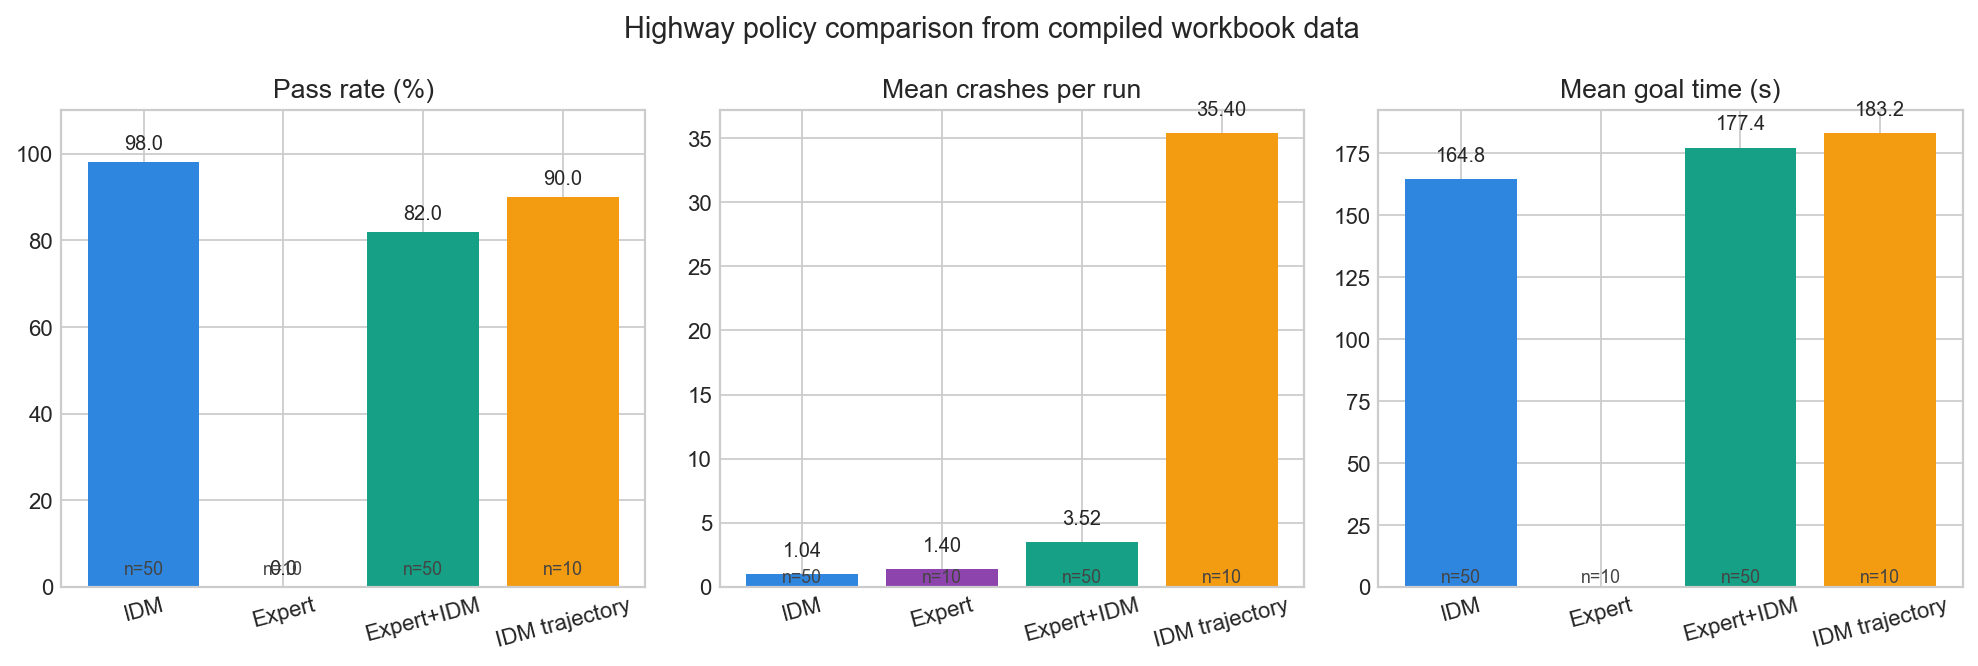
\includegraphics[width=\textwidth]{highway_policy_overview.png}
    \caption{Workbook-derived highway policy comparison}
    \label{fig:highway_overview}
\end{figure}

\begin{figure}[H]
    \centering
    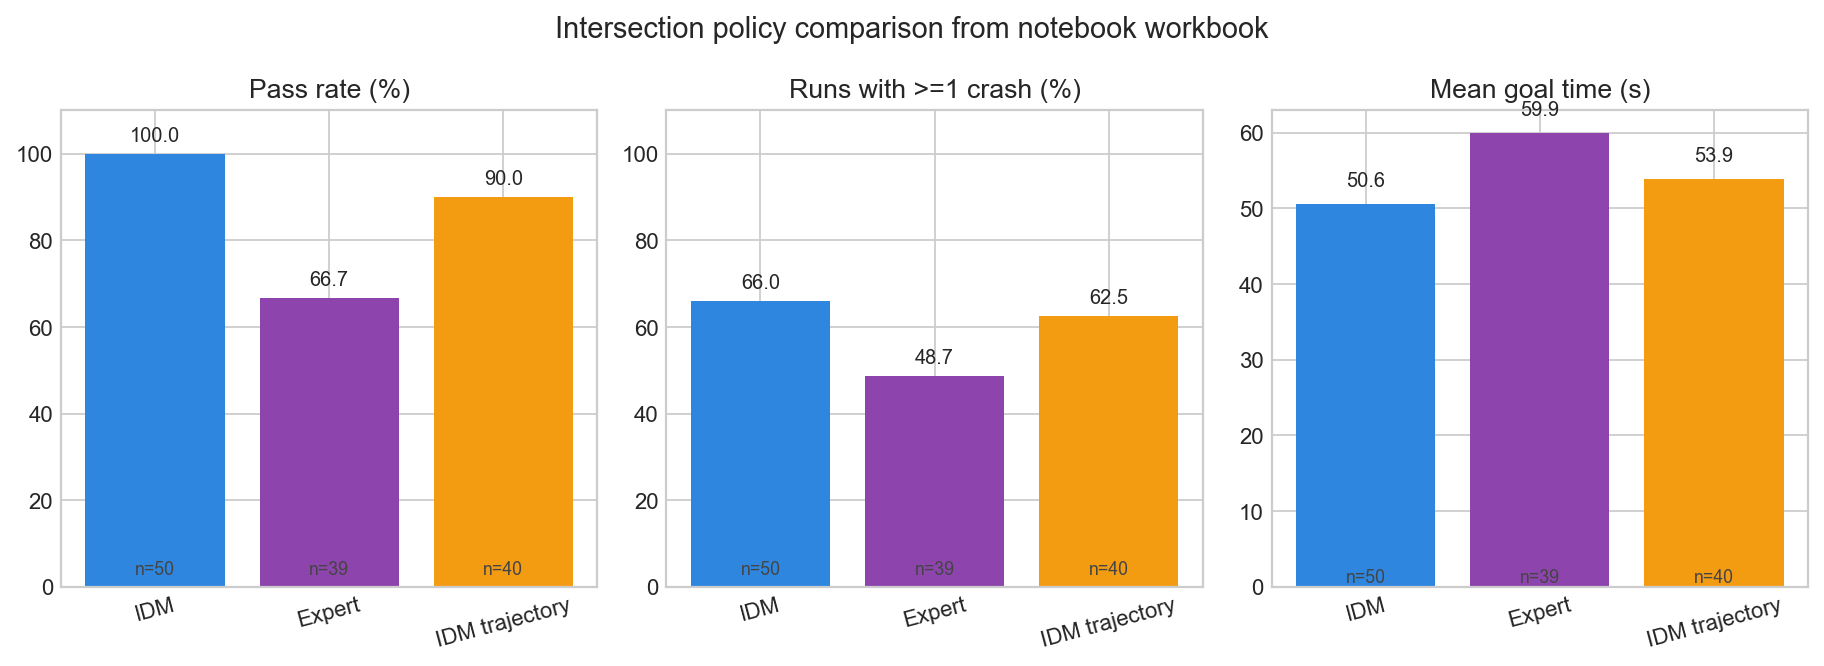
\includegraphics[width=\textwidth]{intersection_policy_overview.png}
    \caption{Workbook-derived comparison for the intersection-roundabout scenario}
    \label{fig:intersection_overview}
\end{figure}

\begin{figure}[H]
    \centering
    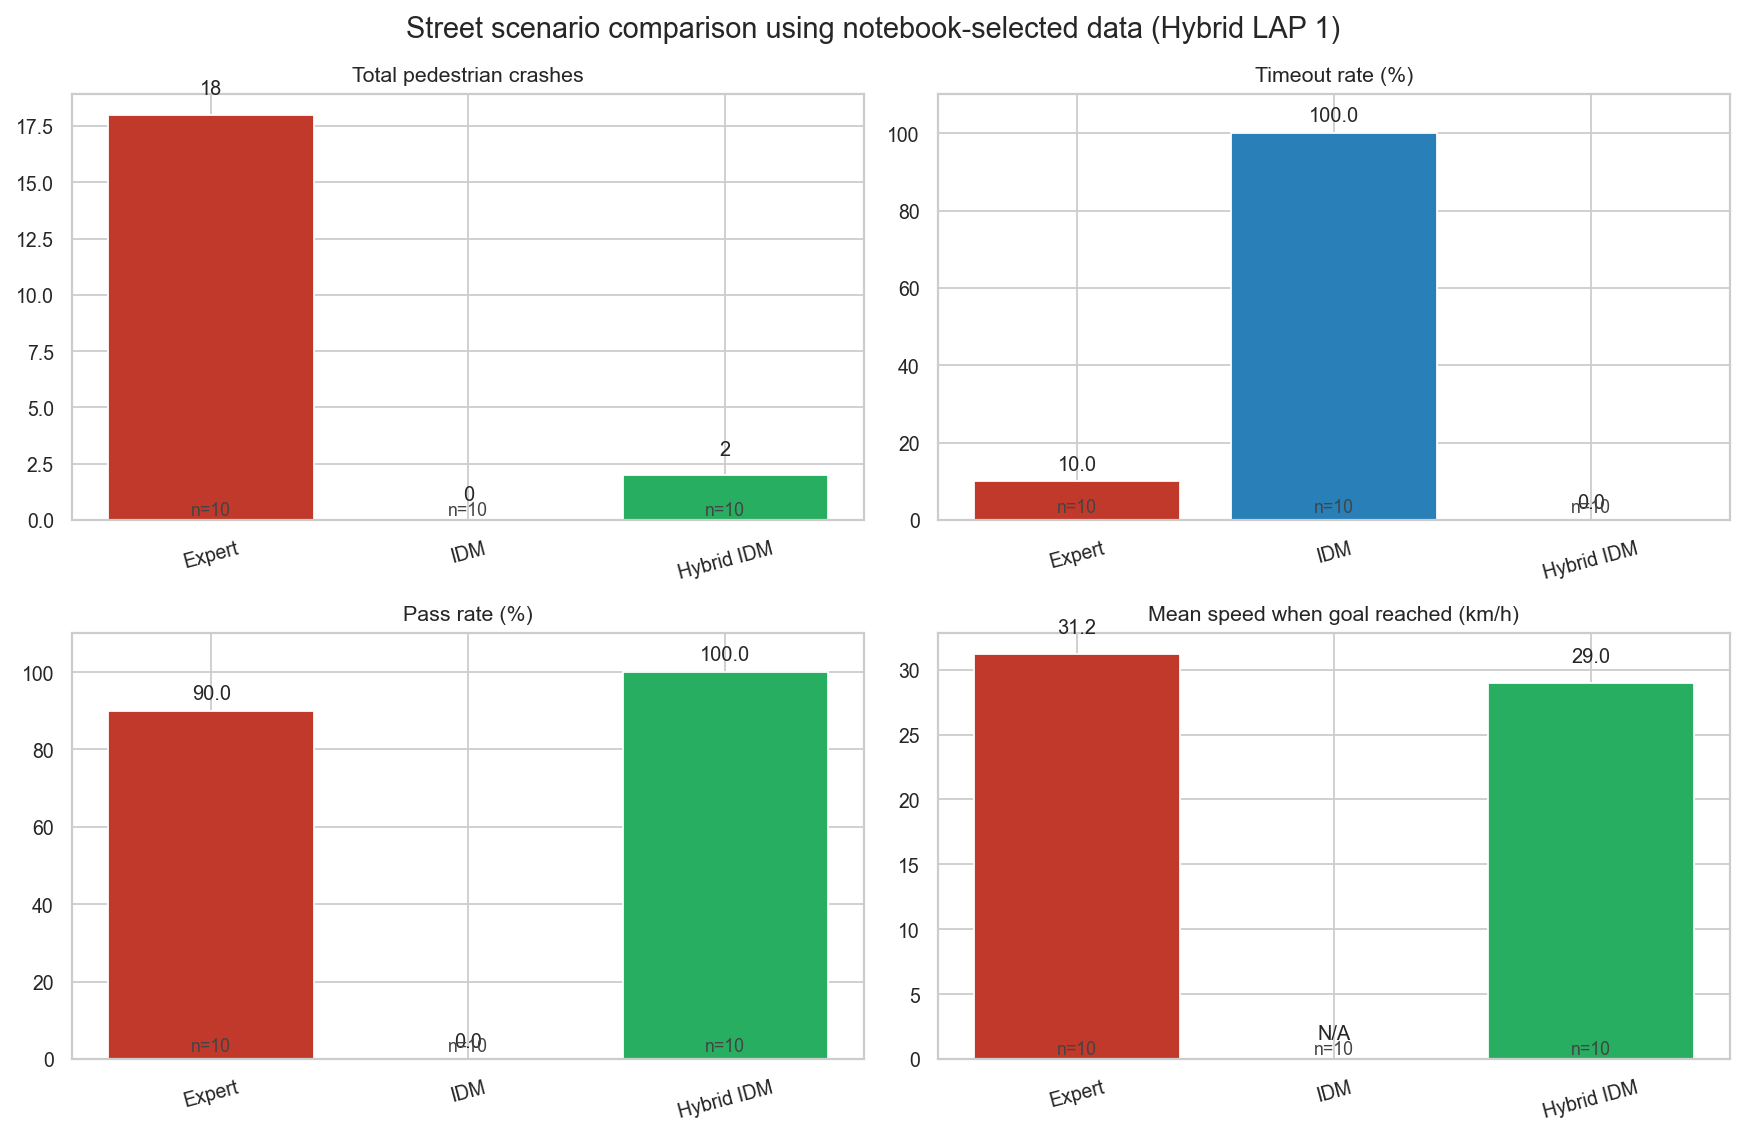
\includegraphics[width=\textwidth]{street_policy_comparison.png}
    \caption{Workbook-derived street policy comparison}
    \label{fig:street_overview}
\end{figure}

\section{Highway Scenario Discussion}

\subsection{Analytical Objective of the Highway Evaluation}
The highway scenario was used to test whether a controller could keep moving on a fixed route while handling traffic and accident-related blockage. In practical terms, the project wanted to know:

\begin{enumerate}[label=\arabic*.]
    \item whether Expert could handle the highway reliably,
    \item whether IDM was too simple for the task,
    \item whether a recovery wrapper could rescue Expert, and
    \item whether planned trajectory following could outperform purely reactive control.
\end{enumerate}

\subsection{Development Observations}
The strongest development-stage observation was that Expert did not merely perform slightly worse than IDM. It failed fundamentally in this scenario. In the saved workbook, it recorded \texttt{0.0\%} pass rate and \texttt{100.0\%} timeout rate. Its average speed was only \texttt{3.75 km/h}, which shows that the controller spent most of its time making almost no progress.

This observation directly led to the \texttt{StuckAwareExpertPolicy}. The idea was not invented in abstract. It came from the real development need to rescue a controller that was repeatedly getting trapped.

\subsection{Highway Results and Interpretation}
The consolidated highway comparison shown in Figure~\ref{fig:highway_overview} is used together with the workbook values in Table~\ref{tab:highway_results} for the interpretation below.

IDM is the strongest overall highway controller in the saved dataset. It achieves \texttt{98.0\%} pass rate, only \texttt{2.0\%} timeout rate, the lowest average crash count among the successful policies (\texttt{1.04}), and an average goal time of \texttt{164.82 s}. This shows that a simple reactive controller can outperform more complex-looking alternatives when the scenario rewards steady traffic negotiation.

The Expert+IDM hybrid is a useful engineering result even though it is not the best highway policy overall. It improves pass rate from \texttt{0.0\%} to \texttt{82.0\%}, which means the recovery idea clearly solves the complete non-progress failure of pure Expert. However, it also records \texttt{3.52} average crashes per run and \texttt{18.0\%} timeout rate. In addition, every archived hybrid run is crash-involved at least once. This suggests that the fallback often activates only after the scenario has already become risky.

The trajectory variant is the clearest example of why pass rate alone is not enough. On the surface, \texttt{90.0\%} pass rate looks competitive. However, the mean crash count rises to \texttt{35.40}, and every saved run is crash-involved. The interpretation is straightforward: the controller keeps moving, but it does not interact safely enough with the surrounding traffic and blockage. Therefore, it cannot be judged as a good highway policy even though it often reaches the destination.

\subsection{Summary of Highway Findings}
The highway results answer the project questions clearly:

\begin{itemize}
    \item Expert is not suitable for this highway setup in its tested form.
    \item A recovery wrapper can improve completion, but it does not automatically create safe behaviour.
    \item Planned path following without strong interaction handling can preserve motion while still creating excessive collisions.
    \item IDM is the best highway controller in the current dataset because it gives the best balance between progress and safety-related behaviour.
\end{itemize}

\section{Intersection-Roundabout Scenario Discussion}

\subsection{Analytical Objective of the Junction Evaluation}
The intersection-roundabout scenario was designed to answer a more structured question: when the ego route is fixed and the conflict points are known, does route-aware control become more useful, and how do completion and crash behaviour change?

\subsection{Role of the Junction Scenario in Project Development}
This scenario was also a design milestone. The project moved from using a built-in route style to building a fully custom map. That step mattered because it created a fairer experiment. From this point onward, it was possible to say with confidence that the target agent was facing the same intended route in every run.

\subsection{Intersection-Roundabout Results and Interpretation}
The consolidated junction comparison shown in Figure~\ref{fig:intersection_overview} is used together with the workbook values in Table~\ref{tab:intersection_results} for the interpretation below.

IDM again gives the strongest overall result. It reaches \texttt{100.0\%} pass rate with no timeouts and an average goal time of \texttt{50.60 s}. This means that, under the fixed-route junction task used in this project, IDM combines reliability and reasonable speed very effectively.

At the same time, IDM is not collision-free. About \texttt{66.0\%} of IDM runs contain at least one crash event, and the mean crash count is \texttt{2.82}. This is an important point for the report: completion does not mean perfect safety behaviour.

Expert behaves very differently here compared with the highway. It is no longer a total failure. It achieves \texttt{66.7\%} pass rate and has the lowest mean crash count (\texttt{1.28}) as well as the lowest share of crash-involved runs (\texttt{48.7\%}). This indicates that Expert is more conservative at conflict points. However, that caution comes with a cost: \texttt{23.1\%} timeout rate and the slowest average successful trip time (\texttt{59.94 s}). In simple terms, Expert is gentler, but it is too hesitant to be the strongest overall policy in this scenario.

TrajectoryIDM is the most interesting middle case. It achieves \texttt{90.0\%} pass rate, zero timeouts, and the highest average speed at \texttt{28.35 km/h}. This shows that route-aware control is meaningful here. However, its mean crash count rises to \texttt{5.10}, and \texttt{62.5\%} of its runs contain at least one crash. The likely interpretation is that route knowledge helps it keep moving, but it still does not manage conflict as cleanly as needed.

\subsection{Summary of Junction Findings}
The intersection scenario shows that:

\begin{enumerate}[label=\arabic*.]
    \item route control does improve the fairness of the experiment,
    \item Expert is much more scenario-sensitive than IDM,
    \item trajectory guidance can improve speed and completion without solving safety by itself, and
    \item IDM is still the best overall compromise in the current junction dataset.
\end{enumerate}

This result is important because it shows that the relative quality of a controller cannot be judged from highway tests alone.

\subsection{Role of the PPO Training Workflow}
The PPO training script is a meaningful part of the project process, but it is not included in the final intersection benchmark table because a matching compiled workbook is not part of the archived final comparison. This means the PPO workflow should be treated as an implementation and extension contribution rather than a final benchmark result in this report.

\section{Street Scenario Discussion}

\subsection{Analytical Objective of the Street Evaluation}
The street scenario asked the most safety-critical question in the project: can a controller handle repeated pedestrian interactions while still finishing the route?

This question is more demanding than the highway and intersection questions because it combines mobility and protection of vulnerable road users. A controller that never moves may avoid crashes, but it is not useful. A controller that finishes quickly but hits pedestrians is also unacceptable.

\subsection{Development of the Street Evaluation Concept}
The idea development in the street scenario is especially clear:

\begin{enumerate}[label=\arabic*.]
    \item repeated crosswalk sites were added because one event was not enough,
    \item Expert and IDM were tested and showed opposite weaknesses,
    \item the project then introduced \texttt{PedestrianAwareIDMPolicy} so that pedestrian conflict directly influenced control,
    \item the final comparison checked whether this modification improved the balance between safety and progress.
\end{enumerate}

\subsection{Street Results and Interpretation}
The consolidated street comparison shown in Figure~\ref{fig:street_overview} is used together with the workbook values in Table~\ref{tab:street_results} for the interpretation below.

The street results show the clearest value of a project-specific policy modification.

Expert achieves \texttt{90.0\%} pass rate and is slightly faster than Hybrid IDM when it finishes, with average goal time \texttt{140.26 s}. However, it records \texttt{1.80} pedestrian crashes per episode on average, and \texttt{90.0\%} of runs include at least one pedestrian crash. This means Expert is efficient enough to move through the task, but not safe enough around pedestrians.

Plain IDM shows the opposite extreme. It records zero pedestrian crashes and zero vehicle crashes in the final street workbook, but it also records \texttt{0.0\%} pass rate and \texttt{100.0\%} timeout rate. The saved script logic helps explain this. The IDM batch uses a shorter stuck timeout rule, and the controller appears to become too hesitant near pedestrians. This means it avoids contact partly by failing to continue the route.

Hybrid IDM gives the strongest balance for this street task. Using the \texttt{LAP == 1} filtered rows, it achieves \texttt{100.0\%} pass rate, \texttt{0.0\%} timeout rate, and only \texttt{0.20} pedestrian crashes per episode. Only \texttt{10.0\%} of its analysed runs contain a pedestrian crash. This is a major reduction compared with Expert. The result supports the design intention of the project-authored controller: treating pedestrian conflict as a direct control input changes the measured safety outcome in a meaningful way.

\subsection{Remaining Trade-Offs in the Street Results}
The street result is strong, but it is not perfect. Hybrid IDM records \texttt{4.20} mean vehicle crashes per episode, which is higher than Expert's \texttt{1.00}. This means the hybrid is best interpreted as a targeted improvement for pedestrian-aware street driving, not as a fully superior policy on every axis.

That trade-off is important for the professional quality of the report. The project should not overclaim. The street hybrid clearly improves the balance between mission completion and pedestrian safety, but it still needs better vehicle interaction handling.

\subsection{Interpretation Notes for the Street Results}
Two caveats must be stated clearly:

\begin{enumerate}[label=\arabic*.]
    \item the final Hybrid IDM comparison uses only rows with \texttt{LAP == 1}, and
    \item the IDM street batch uses a different timeout rule from Expert and Hybrid IDM.
\end{enumerate}

These caveats do not remove the value of the result, but they do affect how precisely the pass-rate difference should be interpreted.

\section{Cross-Scenario Synthesis}
When the three scenarios are read together, the project gives a clear overall answer: no controller family dominates every context.

\begin{table}[H]
    \centering
    \small
    \caption{Best policy choice by scenario in the current project}
    \label{tab:best_policy_by_scenario}
    \begin{tabularx}{\textwidth}{>{\raggedright\arraybackslash}p{2.9cm} X X}
        \toprule
        Scenario & Best current choice & Reason \\
        \midrule
        Highway & IDM & Highest completion, lowest timeout, and lowest collision burden among the successful policies \\
        Intersection-roundabout & IDM & Full completion and zero timeout with moderate speed and lower crash burden than TrajectoryIDM \\
        Street & Hybrid IDM & Best balance between route completion and pedestrian protection \\
        \bottomrule
    \end{tabularx}
\end{table}

This synthesis answers the main research questions:

\begin{itemize}
    \item Policy ranking is not stable across scenarios.
    \item A simple reactive baseline can outperform more advanced-seeming options.
    \item Scenario-specific engineering changes can solve real observed failures.
    \item Pass rate alone is not enough; timeout, crash type, speed, and goal time all matter.
\end{itemize}

\section{Main Findings}
The main findings of the project are as follows.

\begin{enumerate}[label=\arabic*.]
    \item \textbf{IDM is the strongest baseline overall.} It is the best choice in the highway and intersection datasets because it balances strong completion with acceptable stability.
    \item \textbf{Expert is highly scenario-sensitive.} It fails completely on the tested highway setup, improves in the intersection scenario, and reaches high completion on the street, but with poor pedestrian safety.
    \item \textbf{Hybrid design helps when it targets a clear failure.} The highway Expert+IDM wrapper solves the worst stagnation issue of Expert. The street Hybrid IDM strongly improves the balance between progress and pedestrian safety.
    \item \textbf{Trajectory guidance helps movement more than safety.} In both highway and intersection settings, trajectory-informed control preserves progress, but its crash behaviour remains a major weakness.
    \item \textbf{Scenario-specific evaluation is necessary.} The same controller family can move from best to poor depending on the scenario type. Therefore, one universal controller conclusion would be misleading.
\end{enumerate}

\chapter{Conclusion and Future Work}

\section{Conclusion}
This project developed a complete MetaDrive-based evaluation framework for autonomous driving policy comparison across highway, intersection-roundabout, and street scenarios. The contribution is not only the use of simulator baselines. It includes custom scenario design, project-authored policy logic, workbook-based experiment logging, and detailed comparative analysis.

The strongest conclusion of the project is that controller quality is scenario-dependent. In the highway and intersection scenarios, plain IDM gives the best overall performance because it balances completion, progress, and interaction stability better than the alternatives in the saved datasets. In the street scenario, the project-authored Hybrid IDM policy gives the best balance between route completion and pedestrian protection. This shows that targeted scenario-specific engineering is meaningful and can produce better results than relying only on default baseline policies.

The project therefore answers its main question in a firm way: there is no single controller in this work that is best for every road context. A strong evaluation framework must expose that fact rather than hide it behind one overall score.

\section{Limitations}
The main limitations of the project are:

\begin{enumerate}[label=\arabic*.]
    \item the work is fully simulation-based,
    \item not every implemented policy has a matching final compiled benchmark,
    \item sample sizes are not fully matched across all policies, and
    \item the street scripts do not all use the same timeout logic.
\end{enumerate}

These limitations should be considered when interpreting the exact numerical advantage of one policy over another.

\section{Future Work}
Several extensions would strengthen the project further.

\begin{enumerate}[label=\arabic*.]
    \item Re-run the street experiments with a fully standardised timeout rule and larger sample sizes.
    \item Add the PPO-trained intersection policy to a consolidated workbook so it can be compared directly with IDM, Expert, and TrajectoryIDM.
    \item Improve the street Hybrid IDM controller to reduce vehicle collisions while preserving pedestrian safety.
    \item Expand the scenario set with denser urban traffic, more varied pedestrian behaviour, and additional road layouts.
    \item Add stronger statistical analysis, such as confidence intervals or significance testing, on top of the current workbook summaries.
\end{enumerate}

The existing framework already provides a good base for these extensions because the scenario construction, logging, and analysis pipeline are in place.

\bibliographystyle{IEEEtran}
\bibliography{references}

\appendix
\chapter{Overleaf Notes}
This folder is prepared as a separate Overleaf-ready package. To use it:

\begin{enumerate}[label=\arabic*.]
    \item Upload the contents of \codefile{test/fyp_report/} to Overleaf.
    \item Name the Overleaf project \texttt{fyp report}.
    \item Set the compiler to \texttt{pdfLaTeX}.
    \item Run BibTeX or use Overleaf auto-compile so the IEEE references resolve.
\end{enumerate}

The package already includes the bibliography and all figures referenced by this document.

\end{document}
